% !TEX root = ../TV-Denoising.tex

\section{Numerical Illustrations}\label{sec:numerics}

In order to illustrate our theoretical findings, we have performed numerical computations on a discretized version of the denoising problem~\eqref{eq-rof}. Let us stress that this section does not provide any theoretical guarantees concerning the geometrical faithfulness of these approximations, and a careful study of the impact of discretization is an interesting avenue for future works. The code to reproduce these results can be found online\footnote{\url{https://github.com/gpeyre/2016-IP-tv-denoising/}}.

%%%
\subsection{Problem discretization}

The problem is discretized on an uniform grid $( (i/n,j/n) )_{i,j=0}^{n-1}$ of $n^2$ points in $[0,1]^2$. For simplicity, we use periodic boundary conditions. The input image $f$ is represented on this grid as $(f_{i,j})_{i,j=1}^n$ and is normalized so that $f_{i,j} \in [0,1]$. The recovered image $(u_{i,j})_{i,j}$ is defined on the same grid. Denoting $y \eqdef f+w$, the problem $\Pp_{\la}(y)$ is then approximated as
\eql{\label{eq-rof-discrete}\tag{$\Pp_\la^d(y)$}
	\umin{u \in \RR^{n^2}} \sum_{i,j=1}^n |u_{i,j}-y_{i,j}|^2 + \la \sum_{i,j}  \norm{\nabla_{i,j} u}
}
where $\norm{\cdot}$ is the Euclidean norm in $\RR^4$.
%
Here, $\nabla_{i,j} u \in \RR^4$ is a 4-fold discretization of the gradient operator, defined as
\eq{
\nabla_{i,j} u = n ( u_{i+1,j}-u_{i,j}, u_{i,j+1}-u_{i,j}, u_{i+1,j+1}-u_{i+1,j}, u_{i+1,j+1}-u_{i,j+1} ) \in \RR^4
}
so that the discrete gradient operator is $\nabla : u \in \RR^{n^2} \mapsto \nabla u \in \RR^{n^2 \times 4}$.
%
We also define the discrete divergence as
\eq{
	\diverg \eqdef -\nabla^\top : \RR^{n^2 \times 4} \rightarrow \RR^{n^2}.
}
%
Note that this differs from the more usual forward  finite-difference approximation (used for instance in~\cite{chambolle2004algorithm}), and we found numerically that this improves the isotropy (rotation invariance) of the scheme. 

%%%
\subsection{Discrete dual problem and iterative algorithm}

We solve the finite dimensional convex optimization problem~\eqref{eq-rof-discrete} using the dual projected gradient descent of~\cite{chambolle2004algorithm}. 
%
It minimizes a discrete counterpart of~\eqref{eq-rof-dual}, which reads
\eql{\label{eq-dual-discr}\tag{$\Dd_\la^d(y)$}
	\umin{z \in \RR^{n^2 \times 4}} \enscond{
		\norm{ \frac{y}{\la} + \diverg(z) }_{\ell^2}
	}{
		z \in \Cc_\infty
	}	
}
\eq{
	\qwhereq
	\Cc_{\infty} \eqdef \enscond{z \in \RR^{n^2 \times 4}}{  
		\foralls (i,j), \norm{z_{i,j}} \leq 1
	}.
}
The solutions $z_\la$ of~\eqref{eq-dual-discr} are in general non-unique because the problem is not strictly convex, but the primal-dual relationship allow one to recovers the unique solution $u_\la$ of the primal problem~\eqref{eq-rof-discrete} as
\eq{
	u_\la \eqdef \diverg(z_\la) + \frac{y}{\la}. 
}

Starting by some initial $z^{(0)} \in \RR^{n^2 \times 4}$, the projected gradient descent reads
\eq{
	z^{(\ell+1)} \eqdef
	\text{Proj}_{\Cc_{\infty}} \pa{
		z^{(\ell)} + \tau \nabla ( \diverg(z) + \frac{y}{\la})
	},
}
where the step size $\tau$ should satisfy $\tau < 2/\norm{\nabla}^2$ where $\norm{\nabla}^2 \le 16 n^2$ %% \todo{check this} this is true with \le 
%% and as n~>\infty, and in some periodic setting with =
 is the operator norm of the gradient. 
%
The orthogonal projection on $\Cc_\infty$ is computed as
\eq{
	\tilde z = \text{Proj}_{\Cc_{\infty}}(z)
	\qwhereq
	\foralls (i,j), \quad
	\tilde z_{i,j} = \frac{z_{i,j}}{ \max( \norm{z_{i,j}}, 1 ) }.
}
%
The $z^{(\ell)} $ converge  toward a solution $z_{\la}$ of~\eqref{eq-dual-discr}, while the primal iterates
\eq{
	u^{(\ell)} \eqdef \diverg(z^{(\ell)}) + \frac{y}{\la} 
}
converge toward the unique solution $u_\la$ of~\eqref{eq-rof-discrete} with a speed $\norm{u_\la-u^{(\ell)}} = O(1/\ell)$ as shown in~\cite{fadili2010tv}.

 

% also outputs a dual vector $z_{\la}$ with $z_{\la,i,j} \in \RR^4$ which satisfies $u-y=\la \diverg(z_\la)$, where $\diverg=-\nabla^\top : \RR^{n^2 \times 4} \rightarrow \RR^{n^2}$ is the discrete divergence. This allows to compute an approximation of a limit dual vector $z_0$ using $z_\la$ for a very small value of $\la$. Note that of course, both $z_\la$ and $z_0$ are non-unique. 

%%%
\subsection{Denoising results}

Figure~\ref{fig-results} displays the solution $u_{\la}$ of~\eqref{eq-rof-discrete} for a set of increasing values of $\la$. We use here $n=512$, and the noise $w$ is a realization of a white noise where each pixel is Gaussian distributed with a variance $\si^2$ for $\si=0.2$.
%
As predicted by Theorem~\ref{thm:spt_stability}, this shows how the level sets of the solution progressively clusters around the extended support Ext$(Df)$ as $\la$ increases. In order to get some insight about the geometry of this extended support, we display the saturation points of $\norm{z_{0}} = (\norm{z_{0,i,j}})_{i,j}$. Note that since $z_0$ is non-unique and we used the one output by the discrete minimization scheme, we do not claim any theoretical guarantee about this procedure. In practice, we observed that starting the algorithm with $z^{(0)}=0$ leads to meaningful results about this extended support, as shown on Figure~\ref{fig-results}.


\newcommand{\myfig}[1]{\includegraphics[width=0.16\textwidth]{figures/#1}}
\newcommand{\figRow}[4]{%
\myfig{#1/original.png}&%
\myfig{#1/noisy-img}&%
\myfig{#1/extended-support.png}&%
\myfig{#1/tv-noisy-#2-ls.png}&%
\myfig{#1/tv-noisy-#3-ls.png}&%
\myfig{#1/tv-noisy-#4-ls.png}\\}

\begin{figure}[H]
\begin{center}
\UseLowRes{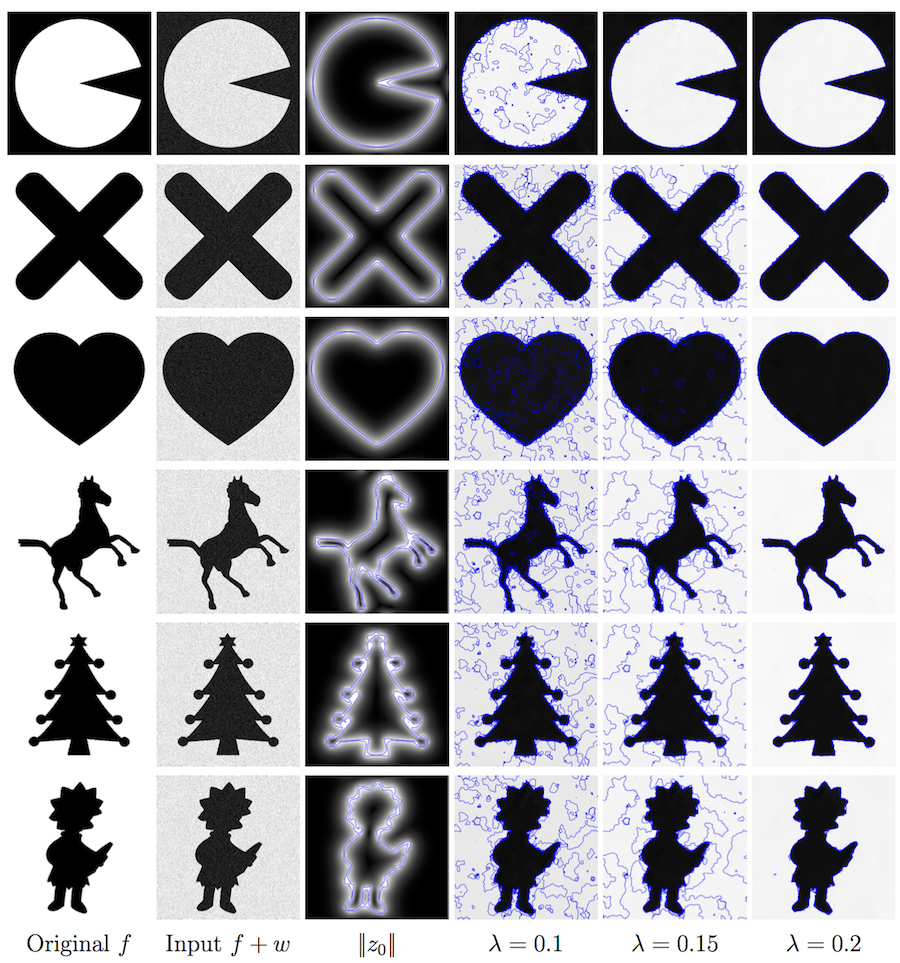
\includegraphics[width=\textwidth]{single.png}
}{
\begin{tabular}{c@{\hspace{1mm}}c@{\hspace{1mm}}c@{\hspace{1mm}}c@{\hspace{1mm}}c@{\hspace{1mm}}c}
%%
\figRow{pacman}{7}{8}{9}
\figRow{cross}{8}{9}{10}
\figRow{heart}{8}{9}{10}
\figRow{horse}{8}{9}{10}
\figRow{sapin}{8}{9}{10}
\figRow{lisa}{8}{9}{10}
Original $f$ & 
Input $f+w$ & 
$\norm{z_0}$  &
$\la=0.1$ & 
$\la=0.15$ & 
$\la=0.2$  
\end{tabular}
}
%%
\caption{\label{fig-results} 
Display of the discretized solution $u_{\la}$ of the discretized problem~\eqref{eq-rof-discrete} for several value of $\la$. The blue curves on top $u_{\la}$ of indicate the level sets of $u_{\la}$ (computed using bilinear interpolation on the grid). The blue curves on top of $\norm{z_0}$ indicate the obtained approximation of the boundary of the extended support Ext$(Df)$.
}
\end{center}
\end{figure}
